\documentclass[spanish]{report}
%%%%%%%%%%%%%%%%%%%%%%%%%%%%%%%%%%%%%%%%%%%%%%%%%%%%%%%%%%%%%%%%%%%%%%%%%%%%%%%%%%%%%%%%%%%%%%%%%%%%%%%%%%%%%%%%%%%%%%%%%%%%%%%%%%%%%%%%%%%%%%%%%%%%%%%%%%%%%%%%%%%%%%%%%%%%%%%%%%%%%%%%%%%%%%%%%%%%%%%%%%%%%%%%%%%%%%%%%%%%%%%%%%%%%%%%%%%%%%%%%%%%%%%%%%%%
\usepackage{amsfonts}
\usepackage{amssymb}
\usepackage[spanish,activeacute, es-tabla]{babel}
\usepackage[utf8]{inputenc}
\usepackage[T1]{fontenc}
\usepackage{graphicx}
\usepackage{float}
%\usepackage[latin1]{inputenc}
\usepackage{amssymb,amsmath} % Formulas matematicas
\usepackage{enumerate}
\usepackage{array}
\usepackage{latexsym}
\usepackage{amsfonts}
%\usepackage{graphicx}
%\usepackage{amsmath}
\usepackage{tocbibind}
\usepackage{nopageno}
\usepackage{fancyhdr}
%\usepackage{graphicx}
\usepackage{multirow}
\usepackage{float}

%%%%%%%%%%%%%%%%%%%%%%%
\setcounter{chapter}{14}
%%%%%%%%%%%%%%%%%%%%%%

%$%%%%%%%%%%%%%%%%%%%%%%%%%%%%%%%%%%%%%%%%%%%%%%%%%%%%%%%%%%%%%%%%%%%%%%%%%%%%%%%%%%%%%%%%%%
%% aqui definimos el encabezado de las paginas pares e impares.
\chead[kk]{Teoría y Aplicaciones en Probabilidad y Estadística}
%\rhead[hdhdhdh]{nada}
\renewcommand{\headrulewidth}{0.5pt}

% aqui definimos el pie de pagina de las paginas pares e impares.

\cfoot[\thepage]{\thepage}
\rfoot[]{}

\renewcommand{\footrulewidth}{0.5pt}

%aqui definimos el encabezado y pie de pagina de la pagina inicial de un capitulo.
\fancypagestyle{plain}{
	\fancyhead[R]{ }
	\fancyhead[L]{ }
	\renewcommand{\headrulewidth}{0.5pt}
	\renewcommand{\footrulewidth}{0.5pt}
}

\pagestyle{fancy}

%%%%%%%%%%%%%%%%%%%%%%%%%%%%%%%%%%%%%%%%%%%%%%%%%

\setcounter{MaxMatrixCols}{10}
%TCIDATA{OutputFilter=LATEX.DLL}
%TCIDATA{Version=5.50.0.2890}
%TCIDATA{<META NAME="SaveForMode" CONTENT="1">}
%TCIDATA{BibliographyScheme=Manual}
%TCIDATA{Created=Saturday, April 28, 2007 15:13:13}
%TCIDATA{LastRevised=Monday, January 27, 2014 20:17:17}
%TCIDATA{<META NAME="GraphicsSave" CONTENT="32">}
%TCIDATA{<META NAME="DocumentShell" CONTENT="Style Editor\Article - LaTeX-like Article">}
%TCIDATA{CSTFile=article.cst}

\setlength{\topmargin}{-0.5in} \setlength{\textheight}{8.0in}
\setlength{\textwidth}{5.0in}
%BeginExpansion
\selectlanguage{spanish}
\newtheorem{theorem}{Teorema}[section]
\newtheorem{acknowledgement}[theorem]{Acknowledgement}
\newtheorem{algorithm}[theorem]{Algoritmo}
\newtheorem{axiom}[theorem]{Suposici\'on}
\newtheorem{case}[theorem]{Caso}
\newtheorem{claim}[theorem]{Ayuda}
\newtheorem{conclusion}[theorem]{Conclusi\'on}
\newtheorem{condition}[theorem]{Condici\'on}
\newtheorem{conjecture}[theorem]{Conjetura}
\newtheorem{corollary}[theorem]{Corolario}
\newtheorem{criterion}[theorem]{Criterio}
\newtheorem{definition}[theorem]{Definici\'on}
\newtheorem{example}[theorem]{Ejemplo}
\newtheorem{exercise}[theorem]{Ejercicio}
\newtheorem{lemma}[theorem]{Lema}
\newtheorem{notation}[theorem]{Notaci\'on}
\newtheorem{problem}[theorem]{Problema}
\newtheorem{proposition}[theorem]{Proposici\'on}
\newtheorem{remark}[theorem]{Observaci\'on}
\newtheorem{solution}[theorem]{Solution}
\newtheorem{summary}[theorem]{Summary}
\newenvironment{proof}[1][Demostraci\'on]{\textbf{#1.} }{\ \rule{0.5em}{0.5em}}
\unaccentedoperators \unspacedoperators \selectspanish
%EndExpansion
\hyphenation{cre-ci-mien-to pro-ble-ma de-ter-mi-nis-ta va-lor
	va-lo-res di-fe-ren-cia-bi-li-dad si-guien-tes es-ta-cio-na-ria
	pro-ba-bi-li-dad nues-tras nues-tros pro-ce-di-mien-to ge-ne-ral
	fi-na-li-dad ne-ce-sa-ria-men-te ma-ne-ra e-va-lua-ra con-ti-nua
	equi-va-len-te de-ter-mi-nis-tas e-jem-plos es-pe-ra-mos
	in-de-pen-dien-tes re-com-pen-sas si-guien-te ge-ne-ra-les
	re-com-pen-sa su-pon-ga-mos accio-nes nu-me-ra-ble sa-tis-fa-cen
	eu-cli-dia-nos ti-tu-la-da par-ti-cu-lar si-guien-te con-fe-ren-ce
	mo-dels es-ta-cio-na-rias ope-ra-dor ite-ra-ci-on de-sa-rro-lla-da}
%\pagenumbering{gobble}


\pagestyle{plain}

\begin{document}

\setcounter{page}{197}






%\newline

\begin{flushright}

{\Huge Cap\'itulo 14}
\end{flushright}
%\\

\rule{123mm}{.4mm}
\\

%\vspace{1cm}

%\\
%\\
\begin{center}
    PROPUESTA DE MEJORA A LAS ECUACIONES UTLIZADAS EN LA PREDICCION DE LAS FASES MINERALES DEL CLINKER EN CCSA
\end{center}
\vspace{.5cm}
\\

\textbf{Dr. Bulmaro Juárez-Hernández,  Lic. Carlos Alberto Alvarez Bravo}\\

\rule{123mm}{.4mm}
\begin{center}

%\\


%\\
Facultad de Ciencias F\'isico Matem\'aticas,\\
Benem\'erita Universidad Aut\'onoma de Puebla,\\
bjuarez@fcfm.buap.mx, caalvarezbravo@gmail.com
\end{center}



\textbf{Resumen. }
La modelación estadística ha sido ampliamente utilizada en múltiples aplicaciones articulando aspectos teóricos, metodológicos y computacionales. Con anterioridad, en la empresa Cementos Cienfuegos S.A (CCSA), de la provincia de Cienfuegos, Cuba, se han realizado investigaciones con el propósito de obtener ecuaciones para predecir los porcentajes de las fases minerales del clínker producido en el horno 3 de dicha industria. En esta industria se utilizan ecuaciones de Bogue modificadas para calcular los porcentajes de las fases minerales del clínker a partir de los principales óxidos en la harina, las que sobrestiman o subestiman el porcentaje real de las fases minerales en el clínker. Estas ecuaciones se han obtenido por intermedio del Análisis de regresión lineal, previo análisis exploratorio de los datos y haciendo uso del software Statgraphics Centurion XV pero no tienen en cuenta otras variables que están presentes en el proceso, por tanto el presente documento presenta una propuesta para la mejora de las ecuaciones usadas en la actualidad en CCSA.
\vspace{.5cm}
\\

\textbf{Abstract.} Statistical modeling has been widely used in multiple applications articulating theoretical, methodological and computational aspects. Previously, at the company Cementos Cienfuegos S.A (CCSA), in the province of Cienfuegos, Cuba, research has been carried out with the purpose of obtaining equations to predict the percentages of the mineral phases of the clinker produced in kiln 3 of said industry. In this industry, modified Bogue equations are used to calculate the percentages of the mineral phases of the clinker from the main oxides in the flour, which overestimate or underestimate the true percentage of the mineral phases in the clinker. These equations have been obtained through linear regression analysis, after exploratory analysis of the data and using the Statgraphics Centurion XV software, but they do not take into account other variables that are present in the process, therefore this document presents a proposal for the improvement of the equations currently used in CCSA.\\
\vspace{.5cm}
\\
\emph{Palabras clave: } Modelación estadística, clínker, ecuaciones de predicción del clínker.

\section{Introducci\'on}
 El cemento es uno de los principales materiales utilizados en la industria de la construcción. La demanda y producción a nivel mundial tiene diferentes comportamientos de acuerdo con la región y el desarrollo de los diferentes países. El proceso de clinkerización es la parte más importante del proceso de fabricación de cemento que deriva en emisiones atmosféricas que afectan el medio ambiente, por lo que la eficiencia en este proceso es fundamental para reducir dichas emisiones. Investigadores en esta temática como Condezo \cite{condezo2020modelamiento}, Tobón y López \cite{tobon2007replanteamiento}, plantean que el proceso de clinkerización consiste en llevar la harina cruda homogenizada al horno rotatorio a altas temperaturas. En la salida del horno se produce la fusión de varios componentes y se forman gránulos conocidos como clínker. La calidad del clínker a la salida del horno depende de la temperatura de este, el tiempo de residencia de la harina en el horno, la granulometría y la correcta composición de los óxidos:  CaO, Fe2O3, Si2O, SO3 y el Al2O3. 

En la industria cementera cubana Cementos Cienfuegos SA (CCSA) algunos de estos parámetros son garantizados por las instalaciones supervisadas mediante el proceso de control de calidad en el laboratorio de la planta. Las principales fases en el clínker son: alita (C3S), belita (C2S), celita (C3A) y ferrita (C4AF), además, pueden estar presente cristales de cal libre, periclasa y sulfatos alcalinos, entre otros \cite{tobon2007replanteamiento}. Las proporciones, la cristalinidad y la textura de estas fases minerales en el clínker controlan propiedades tan importantes en el cemento como: fraguado, calor de hidratación, reactividad y desarrollo de resistencias \cite{holderbank1975} \cite{glasser1998burning}. De ahí la importancia de cuantificarlas con precisión. Alvarez, Cortes y Moreira \cite{cortes2017metodo}, elaboraron un método a partir del cual se obtiene un grupo de ecuaciones para el cálculo de los porcentajes de las fases minerales del clínker antes de la obtención de dicho producto utilizando los porcentajes de los óxidos en la materia prima ´ mediante las ecuaciones de Bogue las que sobrestiman o subestiman el porcentaje real de las fases minerales en el clínker. Por otra parte Cabrera, Rodríguez y Alvarez \cite{alvarez2021perfeccionamiento} proponen un procedimiento para perfeccionar las ecuaciones propuestas por Alvarez, Cortes y Moreira para CCSA pero estas ecuaciones asumen en su formulación que los porcentajes de los óxidos CaO, SiO2, Al2O3, Fe2O3 y SO3 en el clínker solo dependen de los porcentajes de estos mismos en la harina cuando en realidad se reporta que estos también dependen de la temperatura del horno, el tiempo de residencia de la harina en el horno y la granulometría por solo mencionar algunos parámetros. En ese sentido es objetivo de este estudio hacer una propuesta para la mejora de las ecuaciones usadas en la actualidad en CCSA para el cálculo de los porcentajes de las fases minerales del clínker.


\section{Métodos y ecuaciones de predicción para el cálculo de los porcentajes de las fases minerales del clínker en CCSA}
Varias son las metodologías desarrolladas para la cuantificación de los porcentajes de las fases minerales del clínker, entre ellas las más usadas son: La difracción de Rayos–X (ASTM C1365-98), el Cálculo potencial de Bogue (ASTM C150-94) y la Microscopía óptica \cite{holderbank1975}, \cite{calderon77}, \cite{camara1988analise}. En Tobón y López \cite{tobon2007replanteamiento}, también se habla del Conteo manual de puntos ASTM y García - Márquez \cite{garcia2003automatic} comenta sobre el Análisis digital de imágenes. Es preciso destacar que para el caso de CCSA el algoritmo planteado por Alvarez, Cortes y Moreira, considera la obtención de 5 ecuaciones que permiten predecir los porcentajes de los principales óxidos en el clínker a partir del conocimiento de los porcentajes de estos óxidos en la harina. Estas ecuaciones son las siguientes:
\begin{align}
C3S = 4.071CaO−(7.6SiO2+6.718Al2O3+1.43Fe2O3+2.852SO3) \\  
C2S = 2.867SiO2 − 0.7544C3S  \\                            C3A = 2.65Al2O3 − 1.692Fe2O3   \\                          C4AF = 3.043Fe2O3
\end{align}
Las ecuaciones anteriores usan en su formulación las ecuaciones de Bogue, las cuales sobrestiman o subestiman el porcentaje real de las fases minerales en el clínker por tal razón Cabrera, Rodríguez y Alvarez \cite{alvarez2021perfeccionamiento} proponen un procedimiento para perfeccionar las ecuaciones propuestas por Alvarez, Cortes y Moreira para CCSA. A continuación, se expone dicho procedimiento.

\subsection{Procedimiento para la determinación de las ecuaciones de predicción}
Se propuso un procedimiento para el ajuste del modelo de regresión, donde se comprueban supuestos del Método de Mínimos Cuadrados. El Método de Mínimos Cuadrados Ordinarios ofrece algunas propiedades estadísticas muy atractivas por lo que se considera uno de los métodos más efectivos y populares \cite{damodar2010econometria}. Desde el punto de vista de Harrel \cite{harrell2012regression}, este modelo se usa con frecuencia y sus parámetros se interpretan fácilmente sobre todo después de linealizar el modelo. Dicho procedimiento se organizó metodológicamente en tres etapas para la obtención de las ecuaciones predictivas:\\
Etapa 1- Recopilación de la información y preparación de los datos. \\
Etapa 2- Obtención de las ecuaciones de ajuste para las fases minerales del clínker. \\
Etapa 3- Validación de las ecuaciones de ajuste.\\
En la Etapa 1 fueron considerados dos momentos: la selección de la muestra y el Análisis Exploratorio de Datos (EDA), en el que se integraron el análisis gráfico, la detección de atípicos y el análisis descriptivo. En la Etapa 2, las ecuaciones de ajuste fueron determinadas por el Análisis de Regresión Lineal partiendo de la verificación de supuestos necesarios, el Análisis de correlación y finalmente la estimación de las ecuaciones para los porcentajes de las 4 fases (Alita, Belita, Celita y Ferrita) a partir de las ecuaciones ya validadas por Alvarez, Cortes y Rodríguez \cite{alvarez2019ecuaciones}. La obtención de las ecuaciones de ajuste para las cuatro fases minerales del clínker se realizó por el método Paso a Paso, de acuerdo con Walpole, Myer y Myer \cite{walpole1999probabilidad}, que justifica el modelo final seleccionado. En la Etapa 3. De acuerdo con lo descrito por Garcıa-Marquez \cite{garcia2003automatic}, son varios los métodos y coeficientes que pueden utilizarse para validar las ecuaciones de regresión entre ellos se utilizó la Prueba de la regresión múltiple, el cálculo de los coeficientes de determinación $R^2$ y $R^2$ ajustado y los errores estándar. Otra forma de verificar el ajuste de las ecuaciones obtenidas es mediante el análisis de residuos, de manera gráfica o analíticamente, mediante diferentes pruebas como la Durbin Watson, para determinar si hay correlación significativa basada en el orden en el que se presentan en el archivo de datos.
\subsection{Resultados del procedimiento}
En Alvarez, Cortes y Rodríguez \cite{alvarez2019ecuaciones}, se han determinado las relaciones funcionales existentes entre los porcentajes de los óxidos en el clínker y en la harina. \\

\textbf{Resultados de la Etapa 1. Recopilación de la información y preparación de los datos}\\

La muestra estuvo conformada por 909 observaciones recogidas durante el período comprendido entre Mayo 2019 y Agosto 2019 en el horno 3, único en funcionamiento en CCSA. Del análisis visual para los óxidos en el clínker que ofrece el EDA, pueden observarse valores atípicos según los gráficos de caja de cada uno de los óxidos en el clínker (figura 14.1). Se detectaron valores atípicos donde resaltan varios valores por debajo del cuartil 25 y por encima del cuartil 75. De este análisis se detectaron 4 valores atípicos correspondientes al dióxido de sílice (SiO2), 6 en la variable oxido de aluminio (Al2O3), 2 casos en la variable óxido de hierro (Fe2O3), 6 casos en la variable oxido de calcio (CaO) y 15 casos en el trioxido de azufre (SO3). Sin embargo, el tratamiento dado a los valores atípicos encontrados, por no ser valores extremos, fue sustituirlos por la trimedia o media recortada al 5 un estimador robusto que suaviza el valor de los extremos y es poco sensible a las desviaciones de los supuestos inherentes a los modelos probabilísticos \cite{blanxart1992analisis}. Por las mismas razones en el análisis descriptivo fue utilizado como índice de localización la media recortada o trimedia. A partir de estas consideraciones se obtienen rangos intercuartílicos aceptables en cada uno de los óxidos como se observa en la tabla 1 que serán las variables predictoras para la obtención de los modelos de ajuste. Del propio análisis descriptivo, fueron visualmente contrastados los valores promedio (trimedia) y rango intercuartílico de los 5 óxidos en el clínker con los valores típicos según las especificaciones técnicas del clínker, según criterio de Valle \cite{valle2019modelo}, quien hace referencia a la importancia del control de la calidad de sus parámetros químicos y físicos para respaldar que el producto que se pone a disposición de los clientes cumpla con los parámetros establecidos. De este análisis se observan en general aproximados a los promedios obtenidos, con excepción del SO3 cuyos promedios y rangos de variación están más alejados y en el caso del Fe2O3 supera el cuartil superior. Estas reflexiones permiten presumir que luego de las transformaciones realizadas a los valores atípicos se logra mayor concentración de valores hacia el promedio y menos variabilidad. (Tabla 1).\\

\begin{figure}[h]
    \centering
    \includegraphics[width=1\linewidth]{Sin título.jpg}
    \caption{Gráficos de caja de óxidos en el clinker}
    \label{fig:enter-label}
\end{figure}

\begin{figure}[h]
    \centering
    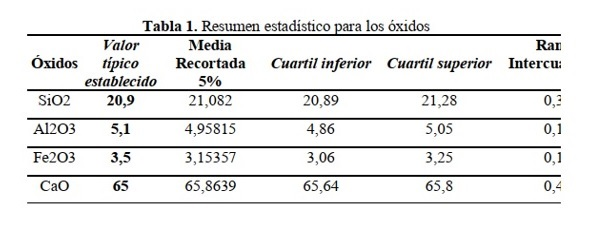
\includegraphics[width=1\linewidth]{Fig.jpg}
    \caption{Resumen estadístico para los óxidos}
    \label{fig:enter-label}
\end{figure}

\textbf{Resultados de la Etapa 2. Obtención de las ecuaciones de ajuste}\\

La obtención de las ecuaciones de ajuste para las cuatro fases minerales del clínker se realizó por el método Paso a Paso que justifica el modelo final seleccionado. \\

\textbf{Verificación de los supuestos}\\

La verificación de la normalidad en las variables dependientes se realizó por intermedio de la Prueba de Anderson-Darling, comprobándose este requisito según la contrastación de las probabilidades asintóticas correspondientes al estadígrafo las que son todas superiores al 5 \% (nivel de significación prefijado), la menor de ellas se obtuvo en la Ferrita (p=0,068), además se comprobó mediante el análisis del sesgo y la curtosis estandarizadas mostradas con anterioridad.\\

Las correlaciones bivariadas por mediación del coeficiente de correlación de Pearson, no mostraron en su generalidad altas correlaciones, sin embargo, al realizar la Prueba T se pudo constatar que todas las correlaciones, aunque no sean tan altas ni tan fuertes, son significativas y ello es suficiente para encontrar ecuaciones ajustadas que permitan predecir el valor estimado de cada una de las fases del clínker en función de sus principales óxidos con un nivel de confianza del 95 \%.\\

\begin{figure}[h]
    \centering
    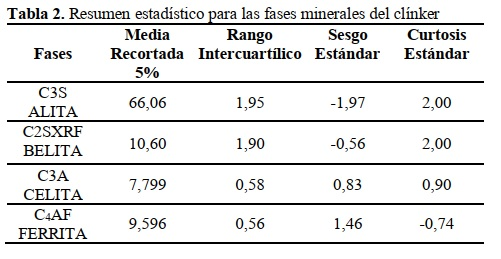
\includegraphics[width=1\linewidth]{Fig 2.jpg}
    \caption{Resumen estadístico para las fases minerales}
    \label{fig:enter-label}
\end{figure}

\textbf{Estimación de ecuaciones}\\

De los análisis de regresión según el método Paso a paso, de cada fase con los óxidos del clínker se obtienen en todos los casos altas correlaciones con coeficientes de determinación mayores que 0,97 lo que indica un buen ajuste, mientras con la Prueba de Regresión múltiple en los cuatro análisis para un 5\% de significación prefijado y un valor P nulo, confirma la significación de las variables independientes. El cuadrado medio del error alcanzó en el último paso, (tabla 3) valores que demuestran la fortaleza de los ajustes obtenidos:\\

\begin{figure}[h]
    \centering
    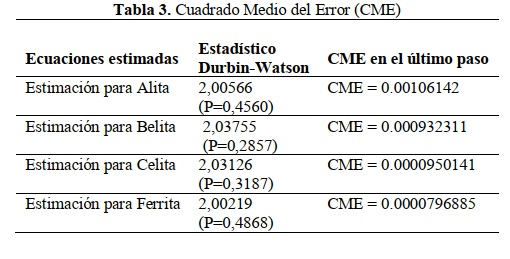
\includegraphics[width=1\linewidth]{Fig 3.jpg}
    \caption{Estadístico D-W y CME}
    \label{fig:enter-label}
\end{figure}

Por su parte el Estadístico Durbin-Watson con (P > 0,05) permite concluir que no existe autocorrelación serial en los residuos con un nivel de confianza del 95 \%. Luego de halladas las ecuaciones para los porcentajes de las 4 fases (Alita, Belita, Celita y Ferrita) fueron
sustituidas en estas, las ecuaciones ya validadas y además comprobada su capacidad de pronóstico por Álvarez, Cortés y Rodríguez [12], para predecir los porcentajes de los principales óxidos en el clínker conociendo los porcentajes de estos óxidos en la harina.\\

Una síntesis de los resultados por pasos se comenta a continuación para cada fase.\\

\textbf{Resultados para la fase C3S: (Alita). Ecuación final ajustada} \\

La ecuación ajustada es la siguiente:
\begin{equation}
    C3S=-0.302242-7.60342SiO2-6.7157Al203-1.41809Fe2O3+4.07575CaO-2.84388SO3
\end{equation}

Luego de sustituir las ecuaciones propuestas por Álvarez, Cortés y Rodríguez en la ecuación ajustada se obtiene:
\begin{equation}
    C3S=87.4606-1.3002SiO2H-6.09979Al203H-1.4280Fe2O3H+0.3952CaOH-1.5401SO3H
\end{equation}

\textbf{Resultados para la fase C2S: (Belita). Ecuación final ajustada}\\

La ecuación ajustada es la siguiente:
\begin{equation}
    C2S=0.266552+8.60333SiO2+5.06538Al203+1.0676Fe2O3-3.07523CaO+2.14447SO3
\end{equation}

Luego de sustituir las ecuaciones propuestas por Álvarez, Cortés y Rodríguez en la ecuación ajustada se obtiene:
\begin{equation}
    C2S=-12.192448+1.4712SiO2H+4.5994Al203H+1.0751Fe2O3H-0.2983CaOH+1.1602SO3H
\end{equation}

\textbf{Resultados para la fase C3A: (Celita). Ecuación final ajustada}\\

La ecuación ajustada es la siguiente:
\begin{equation}
    C3A=-0.0220653+2.65325Al203-1.69004Fe2O3
\end{equation}

Luego de sustituir las ecuaciones propuestas por Álvarez, Cortés y Rodríguez en la ecuación ajustada se obtiene:
\begin{equation}
    C3A=3.5121347+2.4092Al203H-1.7019Fe2O3H
\end{equation}

\textbf{Resultados para la fase C4AF: (Ferrita). Ecuación final ajustada }\\

La ecuación ajustada es la siguiente:
\begin{equation}
    C4AF=0.00190878+3.042237Fe2O3
\end{equation}

Luego de sustituir las ecuaciones propuestas por Álvarez, Cortés y Rodríguez en la ecuación ajustada se obtiene:
\begin{equation}
    C4AF=3.9661+3.0637Fe2O3H
\end{equation}

La valoración del ajuste de los modelos obtenidos se realiza de acuerdo con las especificaciones del procedimiento propuesto, teniendo en cuenta, los resultados de la Prueba de la Regresión Múltiple para contrastar los coeficientes de las variables independientes, la Prueba estadística de Durbin-Watson para conocer la posible presencia de autocorrelación en los de residuos y por último la interpretación de los coeficientes de determinación $R^2$ y $R^2$ modificado.


\section{Problemas presentados por los métodos y procedimientos para el cálculo y predicción de las fases minerales del clínker}

Como se comentó con anterioridad para la cuantificación de los porcentajes de las fases minerales del clínker se han desarrollado varios métodos entre los que se destacan la Difracción de Rayos–X, químico–Cálculo Potencial de Bogue \cite{clark2002bogue} y  microscopía óptica \cite{holderbank1975},\cite{calderon77}, \cite{fundal1980microscopy}, \cite{camara1988analise}. Este último, se realiza  mediante conteo manual de puntos \cite{C1356M-96} o análisis digital de Imágenes \cite{garcia2003automatic}. Es importante decir que todos estos métodos trabajan sobre el clínker ya producido por tanto dichos métodos no garantizan la calidad del clínker a la salida del horno.\\

En Cuba (según los especialistas de la empresa CCSA) y el mundo el método clásico de cuantificar los porcentajes de los minerales del clínker es usando las ecuaciones propuestas por Bogué hace cerca de un siglo \cite{tobon2007replanteamiento}, conocidas como Cálculo Potencial de Bogue. El Cálculo Potencial de Bogue desarrollado por R. H. Bogue consiste en un proceso de cálculo según el cual, a partir del análisis químico, se puede calcular el contenido en minerales del clínker (en porcentaje), sobre todo, de Alita, Belita, Celita y Ferrita. A las ecuaciones encontradas por Bogue se les conoce en la actualidad como las “Ecuaciones de Bogue” \cite{duda2021manual}.\\

El cálculo se realiza a partir del conocimiento de los porcentajes de los principales óxidos que están presentes en el clínker.  En su formulación estas  ecuaciones asumen materias primas con pureza y reacción entre ellas del 100\%, lo cual no es cierto para la mayoría de las cementeras, donde se tienen diferentes combinaciones de materias primas y procesos de clinkerización no totalmente controlados. Además el error se incrementa por la formación de compuestos menores y por la presencia de soluciones sólidas entre los componentes principales y menores \cite{lawrence1998constitution}.
Taylor \cite{taylor1997cement} y otros muestran como algunos investigadores han concluido que los cálculos con las ecuaciones de Bogué generalmente subestiman el contenido de alita y sobreestiman el de belita y celita hasta en un 10\% agregando, que el conteo de puntos mediante microscopía óptica puede producir un resultado más preciso para estas fases.\\

Autores como Crumbie \cite{crumbie2006iron} identifican como una dificultad en el método óptico la cuantificación de los aluminatos (celitas) y ferroaluminatos (ferritas) presentes en la fase intersticial debido principalmente al tamaño tan pequeño de los cristales, los cuales pueden llegar incluso a ser amorfos. Ellos proponen para subsanar esta dificultad el empleo de Difracción de Rayos X Cuantitativa (QXRD) la cual puede ser difícil porque este es un material multifases y varios picos se superponen, sin embargo, ellos plantean que con los desarrollos del método de Rietveld se pueden minimizar o eliminar estos errores, por lo cual autores como Castañón Garcia, Garcia Granda y Guerrero \cite{castanon2012estudio} han reportado el uso de este método.\\

Aceptando que esta dificultad existe, es importante resaltar que una ventaja comparativa que tiene la microscopía óptica sobre estas otras técnicas es que además de cuantificar las fases permite ver las texturas y las alteraciones en los cristales como son: el tamaño de los cristales, distribución de las fases dentro de la muestra, cluster, retrogradaciones, zonaciones, maclas, etc. \cite{campbell1999microscopical} y ahora con el desarrollo de sistemas de análisis digital de imágenes (ADI) esto se puede hacer en muy corto tiempo \cite{garcia2003automatic}.\\

Como se dijo con anterioridad el cálculo del contenido en minerales del clínker mediante las Ecuaciones de Bogue se realiza a partir del conocimiento de la composición de los principales óxidos (CaO, SiO2, Al2O3, Fe2O3 y SO3) en el clínker ya producido, por tanto si se tiene en cuenta la capacidad de producción de los hornos instalados en las industrias cementeras actuales (con una significativa inercia) seria de interés para los especialistas realizar el cálculo antes de la obtención del clínker como base para la toma de decisiones en el proceso de producción de este producto. De esta forma, se garantiza la calidad del producto y una disminución de las pérdidas por producciones fuera de las especificaciones del cliente.\\

En investigaciones anteriores algunos autores como Alvarez Bravo, Cortés Cortés, Moreira Quiñones y Flores Huilcapi, Carrera Almendáriz y Rodríguez Pinos \cite{huilcapi2020analisis} han trabajado en función de obtener o modificar las fases minerales del clínker o algunas de estas antes de que se produzca dicho producto. \\

Alvarez Bravo, Cortés Cortés y Moreira Quiñones plantean la elaboración de un método a partir del cual se obtienen un grupo de ecuaciones para predecir los porcentajes de las fases minerales del clínker producido en la industria cementera cubana Cementos Cienfuegos SA (CCSA) antes de la obtención de dicho producto y utilizando los porcentajes de los óxidos en la materia prima, pero el método utiliza las ecuaciones de Bogue las cuales sobrestiman o subestiman el porcentaje real de las fases minerales en el clínker, debido a que según Tobón y López , estas ecuaciones fueron creadas para calcular el porcentaje de las fases minerales del clínker asumiendo que las materias primas utilizadas tienen una pureza del 100\% y que las reacciones entre ellas son completas, lo cual en la realidad no ocurre y ha llevado durante años a las cementeras a sobrevalorar o subvalorar dichos porcentajes.
Flores Huilcapi, Carrera Almendáriz, y Rodríguez Pinos proponen una metodología para obtener valores deseados de Alita y Belita a partir de la modifcación de manera empírica de los módulos de saturación de cal, sílice y alúmina.\\

Labidi, Boughanmi, Houcine, y Megriche \cite{labidi2019critical} Realizan un estudio crítico de métodos de cuantificación de las fases minerales  mediante una comparación entre el Método de Bogue y el Método de Rietveld demostrando que el último es más fiable que el primero pero como se explicó con anterioridad ambos métodos trabajan sobre el clínker producido. 
Por otra parte Cabrera Alvarez, Rguez Tamayo y Alvarez Bravo proponen un procedimiento para perfeccionar las ecuaciones propuestas por Alvarez Bravo, Cortés Cortés y Moreira Quiñones  para CCSA (procedimiento expuesto anteriormente) a partir de estimar modelos que relacionan los porcentajes de cada óxido en el clínker con los porcentajes de las fases minerales y usando las ecuaciones de predicción de los porcentajes de los óxidos CaO, SiO2, Al2O3, Fe2O3 y SO3 en el clínker propuestas por Álvarez Bravo, Cortés Cortés y Rodríguez Tamayo . Las ecuaciones predictivas encontradas por estos se obtienen por intermedio del Análisis de regresión lineal múltiple, previo análisis exploratorio de los datos. Se utilizó el paquete Statgraphics Centurion XV. Los modelos obtenidos mejoran el porcentaje de ajuste obtenido con anterioridad y fueron validados estadísticamente. Estas últimas ecuaciones asumen en su formulación que los porcentajes de los óxidos CaO, SiO2, Al2O3, Fe2O3 y SO3 en el clínker solo dependen de los porcentajes de estos mismos en la harina cuando en realidad se reporta que estos también dependen de la temperatura del horno, el tiempo de residencia de la harina en el horno y la granulometría por solo mencionar algunos parámetros.\\

En ese sentido y teniendo en cuenta que el horno instalado es de 220 ton/h de clínker (con una significativa inercia) es de interés para los especialistas  de Cementos Cienfuegos realizar el cálculo antes de la obtención del clínker y de la manera más precisa posible, para de esta forma poder hacer correcciones en los gráficos de control del proceso y así evitar elevadas pérdidas económicas por productos fuera de especificaciones, consumo de energía innecesario y emisiones atmosféricas (Información aportada por los especialistas de la empresa), por tanto si los parámetros mencionados son considerados se obtendrá un grupo de ecuaciones para la predicción de las fases minerales del clínker aún más precisas, lo cual podría hacerse empleando métodos  para realizar análisis de regresión tanto clásicos como del ámbito de la inteligencia artificial y comparando cuál de estos ofrece mejores resultados.


\section{Conclusiones}
Los resultados obtenidos hasta ahora para la predicción de las fases minerales del clínker en CCSA constituyen una importante aplicación de la estadística a un problema real con un aporte práctico significativo para esta importante industria. Las cuatro ecuaciones de regresión lineal estimadas por Cabrera Alvarez, Rguez Tamayo y Alvarez Bravo para los porcentajes en las fases minerales del clínker, a partir de las propuestas con anterioridad en CCSA, mejoran el ajuste obtenido hasta el momento con las ecuaciones de Bogue, por lo que son usadas en esta cementera y al ofrecer coeficientes propios para CCSA facilitan la estabilidad en las operaciones del horno, no obstante, estas ecuaciones no tienen en cuenta otras variables presentes en el proceso las cuales al ser consideradas permitirían obtener ecuaciones más precisas para la predicción de las fases minerales del clínker a la vez que contribuirían a la obtención de mejoras en términos de eficiencia en la producción de clínker sobre bases más seguras, con un ahorro de materias primas, portadores energéticos y la disminución de las emisiones de contaminante a la atmósfera, contribuyendo al desarrollo sostenible en la producción de cemento.



%\begin{thebibliography}{9}


%\bibitem{tesisL} Altieri Linda, {\em A Bayesian changepoint analysis on spatio-temporal point processes}, Tesis , 2015.

%\bibitem{Blangiardo} Blangiardo Marta y Cameletti Michela {\em Spatial and Spatio-temporal Bayesian Models with R-INLA}, John Wiley and Sons. 2015.\\

%\bibitem{Chen} Chen, J., y Gupta, A.  {\em Parametric Statistical Changepoint Analysis}, Bogota: Birkhauser. 2012.\\

%\bibitem{Virgilio} G\'omez Rubio Virgilio, {\em Bayesian inference with INLA}, Champman and Hall, 2020.\\

%\bibitem{Jeffreys} Jeffreys H., {\em Theory of probability}, Oxford: Oxford University Press; 1961. \\
%\end{thebibliography}
\bibliographystyle{ieeetr}
\bibliography{Referencias}


\end{document}
